\subsection{Loop antenna}\label{sec:loop_sim}
\subsubsection{Setup}

\FloatBarrier

\begin{figure}[tbp]
	\centering
	\raisebox{-4.5mm}{
	\begin{subfigure}[t]{0.49\textwidth}
		\centering
		\includegraphics[width=1\linewidth]{content/img/loop_near_field}
		\caption{Electric near-field intensity of loop antenna}
		\label{fig:loopnearfield}
	\end{subfigure}
}
	\hfill
	\begin{subfigure}[t]{0.48\textwidth}
		\centering
		\includegraphics[width=1\linewidth]{content/img/loop_antenna}
		\caption{Geometry of loop antenna}
		\label{fig:loopantenna}
	\end{subfigure}
	
	\caption{The geometry of the loop antenna assimilates a square with round edges. The height and width of the antenna equal $h=w=1.6$\,mm. The return path leads back to the PEC surface of the TEM cell. The electric near-field shows large a displacement current and voltage drop near the feed-point. It has been derived with a refined mesh on the antenna surface and near the feedpoint, according to the discussion in \cref{sec:mesh}.}
	\label{fig:loop_moments_phase}
\end{figure}

A loop antenna is the most basic form of an antenna generating a mangetic dipole moment.

A square loop antenna is placed in the center of the TEM cell. It consists of four wires with a length of 1.6\,mm each, and it is electrically short for frequencies up to 4.69\,GHz. The square geometry is preferable to a round version in the numerical simulations, as it allows for more accurate meshes and enables a clearer investigation of the resulting dipole moments. 

The normal vector of the loop surface points in x-direction, leading to a maximum coupling with the magnetic field of the TEM-mode. In contrast to the monopole antenna discussed in \cref{sec:monopole}, a return path for the current exists, which generates a magnetic dipole moment.

\subsubsection{Equivalent dipole moments}\label{sec:eq_dip_loop}
%
%\todo[inline]{TODO: Knowing the loop area, $\mathbf{h}^\pm$ and feed current, could the mag. dipole moment be approximated?}

The equivalent dipole moments of the loop antenna are plotted in \autoref{fig:dipole_moments_loop_antenna}. The magnetic dipole moment $\mathbf{m}_\mathrm{m}$ dominates over the electric dipole moment $\mathbf{m}_\mathrm{e}$. Opposed to the case of a monopole antenna, $\mathbf{m}_\mathrm{e}$ and $\mathbf{m}_\mathrm{m}$ demonstrate non-linear behavior over frequency, which is investigated further in \cref{sec:loop_electrical_characteristics}.

Furthermore, the phases of the powers at the output ports, shown in \autoref{fig:loopphase}, differ from one another. The phase shift in the low-frequency range approaches $\pi$, but gradually decreases with increasing frequency. This agrees with the analysis presented in \cref{sec:equ-dip-mom}, which predicts a phase shift of $\pi$ when only $\mathbf{m}_\mathrm{m}$ is present, and a reduced phase shift as $\mathbf{m}_\mathrm{e}$ increases, as is the case here.

\begin{figure}[tbp]
	\centering
	\begin{subfigure}[t]{0.5\textwidth}
		\centering
		\includegraphics[width=1\linewidth]{content/img/dipole_moments_loop_antenna.png}
		\caption{Equivalent dipole moments}
		\label{fig:dipole_moments_loop_antenna}
	\end{subfigure}
	\hfill
	\begin{subfigure}[t]{0.48\textwidth}
		\centering
		\includegraphics[width=1\linewidth]{content/img/loop_phase}
		\caption{Phase of the power at each output port}
		\label{fig:loopphase}
	\end{subfigure}
	
	\caption{The equivalent dipole moments of the loop antenna are derived analytically with \crefrange{eqn:ifa_me}{eqn:ifa_mm}, where the electric dipole moment $\mathbf{m}_\mathrm{e}$ is weighted with $Z_0$ to enable comparison with $\mathbf{m}_\mathrm{m}$. The phases of the powers at output ports 1 and 2 are derived from the S-parameters, as discussed in \cref{sec:s-param-data}. The analysis specifically focuses on the phase shift between the two ports, which provides information about the presence of $\mathbf{m}_\mathrm{m}$ and $\mathbf{m}_\mathrm{e}$, as investigated in \cref{sec:equ-dip-mom}.}
	\label{fig:loop_moments_phase}
\end{figure}

%The surface of the loop equals $S=1.68\,\mathrm{mm}^2$. The magnetic dipole moment $\mathbf{m}_m$ can be approximated by applying \crefrange{eqn:e_a_closed_int}{eqn:m_v}, using the normalized magnetic field intensity of the TEM mode $\mathbf{h}_\mathrm{TEM}^\pm$ and the feed voltage in \autoref{fig:loopfeedreturncurrent}. At 3\,GHz, for example, this yields
%
%\begin{equation}
%	\mathbf{m}_m (f=3\,\mathrm{GHz})=I()\cdot j\omega \mu_0 \frac{S\cdot(\mathbf{h}^-_\mathrm{TEM} - \mathbf{h}^+_\mathrm{TEM})}{2\mathbf{e}^\pm_\mathrm{TEM}\cdot k_0}
%\end{equation}

The power and $E_y$ induced by the loop antenna at the output ports is shown in \autoref{fig:loopopower}, and increases not as steeply as the output power of the monopole antenna exhibited in \autoref{fig:monopoleoutputpower}. This directly correlates with the decrease of $\mathbf{m}_\mathrm{m}$ with increasing frequency.

\autoref{fig:loopopowercomp} demonstrates the output power generated by the equivalent dipole moments $\mathbf{m}_\mathrm{m}$, $\mathbf{m}_\mathrm{e}$ and the loop antenna. Their similarity support the validity of the model used.

\begin{figure}[tbp]
	\centering
	\begin{subfigure}[b]{0.48\textwidth}
		\centering
		\includegraphics[width=1\linewidth]{content/img/loop_opower}
		\caption{Electric field and output power}
		\label{fig:loopopower}
	\end{subfigure}
	\hfill
	\begin{subfigure}[b]{0.5\textwidth}
		\centering
		\includegraphics[width=1\linewidth]{content/img/loop_opower_comp}
		\caption{Comparison of output powers}
		\label{fig:loopopowercomp}
	\end{subfigure}
	
	\caption{Electric field in y-direction $E_\mathrm{y}$ at $x=0, y=b/4, z=\pm l/2$, and the closely related power at one of the output ports, derived with the S-parameters in \autoref{eqn:power_antenna}. The output power produced by the loop antenna is compared with that generated by the equivalent dipole moments.}
	\label{fig:example}
\end{figure}


\subsubsection{Electrical characteristics}\label{sec:loop_electrical_characteristics}

Calculating the electric and magnetic energy in the radiation boundary, as discussed in \cref{sec:energy-densities-reactances}.




\begin{figure}[htbp]
	\centering
	\includegraphics[width=1\linewidth]{content/img/loop_electromagnetic_energy}
	\caption{Electric and magnetic energy produced by the loop antenna in the TEM cell, derived with \autoref{eqn:em_energy} in the TEM cell volume.}
	\label{fig:loopelectromagneticenergy}
\end{figure}


%
%The output power is calculated through the S-parameters. The impedance too. The voltage and current at the antenna port follow from the impedance and input power. The magnetic and electric energy in the TEM cell is calculated through integrating the electric and magnetic field intensities. By dividing them with the voltage and current, the inductance and capacitance of the antenna is calculated.  \todo{Passt so vermutlich nicht: die port s parameter lügen diesbezüglich ein wenig, da sehr viel strom bereits nähe des ports als displacement current zurückfließt.}



\begin{figure}[tbp]
	\centering
	\begin{subfigure}[t]{0.45\textwidth}
		\centering
		\includegraphics[width=1\linewidth]{content/img/loop_feed_return_current_voltage}
		\caption{Voltage and current}
		\label{fig:loopfeedreturncurrent}
	\end{subfigure}
	\hfill
	\begin{subfigure}[t]{0.45\textwidth}
		\centering
		\includegraphics[width=1\linewidth]{content/img/curr_imp}
		\caption{Impedance}
		\label{fig:currimp}
	\end{subfigure}
	
	\caption{This figure demonstrates the voltage, current and impedance characteristics of the loop antenna. The difference between the current near the feedpoint and that on the return path increases with frequency, indicating a growing occurrence of displacement currents. The current on those paths are determined through magnetic near-field intensity, using \autoref{eqn:ampere_law_fem}. The voltage across the feedpoint is obtained using \autoref{eqn:vin}. Magnitude and phase of the impedance of the loop antenna are determined with \autoref{eqn:za}.}
	\label{fig:example}
\end{figure}


The current $I$ in the loop antenna changes along the antenna wire as shown in \autoref{fig:loopfeedreturncurrent}, indicating displacement current coupling to the septum and back to the feedpoint. The difference between the feedpoint and return path current increases over frequency, translating to rising displacement currents. Furthermore, the decrease in feed current over rising frequency, shown in \autoref{fig:loopfeedreturncurrent}, also hints to the presence of increasing displacement currents. Consequently, $\mathbf{m}_e$ gains a significant magnitude according to \autoref{eqn:me_i}, increasing the electric coupling of the antenna to the TEM cell. 

The feedpoint current is derived with \cref{eqn:ampere_law_fem}, through integration of $\mathbf{H}$ in a closed loop of radius 0.11\,mm, measured 0.17\,mm above the feedpoint. The return path current is processed with the same loop integration at the same height above the PEC surface. The results vary with height above the PEC surface due to the displacement currents in the near-field.

\autoref{fig:loopfeedreturncurrent} demonstrates the voltage at the feedpoint of the antenna, which significantly rises over the frequency, signaling increased induced voltage $V_\mathrm{n}$. According to \autoref{eqn:m_v}, this directly correlates with $\mathbf{m}_\mathrm{m}$, which furthermore becomes apparent when comparing their behavior shown in \crefrange{fig:dipole_moments_loop_antenna}{fig:loopfeedreturncurrent}. The increase in voltage also correlates with the displacement current. It raises the potential on the loop antenna, therefore increasing the charge distributions and displacement currents.

The increases in voltage and decrease in current agrees with the impedance, depicted in \autoref{fig:currimp}. The loop antenna shows strongly inductive behavior. 

\subsubsection{Equivalent circuit model}

Following the same approach established in \cref{sec:monopole_eqc}, an 
equivalent circuit is derived for the small loop antenna. 
\autoref{fig:eqc_balanis} demonstrates the full equivalent circuit for the 
electrically small loop antenna in free space \cite[p. 244]{Balanis_1997}, 
where

\hspace{1cm}\begin{minipage}{\dimexpr\textwidth-2cm}
	\begin{description}
		\item[$C_s$]   Stray capacitance of the loop antenna
		\item[$R_L$]   Ohmic loss resistance of the antenna conductor
		\item[$R_r$]   Radiation resistance of the loop antenna
		\item[$L_i$]   Internal inductance of the loop antenna
		\item[$L_e$]   External inductance of the loop antenna
	\end{description}
\end{minipage}

As discussed in \cref{sec:antenna_model}, the antenna is modeled as a perfect 
electric conductor, therefore $R_L$ and $L_e$ are neglected. Instead, the 
simplified equivalent circuit in \autoref{fig:eqc_simple} is applied, where 
$R_A$, $L_A$ and $C_A$ represent the impedance behavior of the antenna.

\begin{figure}[tbp]
	\centering
	\begin{subfigure}[b]{0.45\textwidth}
		\centering
		\resizebox{0.7\textwidth}{!}{
			\begin{tikzpicture}
				% Paths, nodes and wires:
				\draw (11.75, 6) to[european inductor, l={$L_{i}$}] (9.75, 6);
				\draw (12, 2) to[european inductor, l_={$L_{A}$}] (12, 4);
				\draw (7, 6) to[capacitor, l={$C_s$}] (7, 2);
				\draw (12, 5.75) to[european resistor, l={$R_{r}$}] (12, 3.75);
				\draw (9.25, 6) to[european resistor, l={$R_{L}$}] (7.25, 6);
				\node[ground] at (7, 2){};
				\node[ground] at (12, 2){};
				\draw (7, 6) -- (5, 6);
				\node[circ] at (7, 6){};
				\draw (7, 6) -- (7.25, 6);
				\draw (9.25, 6) -- (10, 6);
				\draw (11.75, 6) -- (12, 6);
				\draw (12, 5.75) -| (12, 6);
				\draw[-latex] (5, 6.5) -- (6.75, 6.5);
				\node[shape=rectangle, minimum width=2.215cm, 
				minimum height=0.965cm] at (6.534, 6.75){} 
				node[anchor=north west, align=left, text width=1.827cm, 
				inner sep=6pt] at (5.409, 7.25){$P_{in}$};
			\end{tikzpicture}
		}
		\caption{Full equivalent circuit \cite[p. 244]{Balanis_1997}}
		\label{fig:eqc_balanis}
	\end{subfigure}
	\hfill
	\hspace*{-0.5cm}
	\begin{subfigure}[b]{0.45\textwidth}
		\centering
		\resizebox{0.65\textwidth}{!}{
			\begin{tikzpicture}
				% Paths, nodes and wires:
				\draw (11, 3) to[european inductor, l_={$L_{e}$}] (11, 5);
				\draw (7, 6) to[capacitor, l={$C_A$}] (7, 2);
				\node[ground] at (7, 2){};
				\node[ground] at (11, 2){};
				\draw (7, 6) -- (5, 6);
				\node[circ] at (7, 6){};
				\draw (7, 6) -- (7.25, 6);
				\draw[-latex] (5, 6.5) -- (6.75, 6.5);
				\node[shape=rectangle, minimum width=2.215cm, 
				minimum height=0.965cm] at (6.534, 6.75){} 
				node[anchor=north west, align=left, text width=1.827cm, 
				inner sep=6pt] at (5.409, 7.25){$P_{in}$};
				\draw (11, 2) -| (11, 3);
				\draw (7.25, 6) to[european resistor, l={$R_A$}] (11, 6);
				\draw (11, 6) -- (11, 5);
			\end{tikzpicture}
		}
		\caption{Reduced equivalent circuit}
		\label{fig:eqc_simple}
	\end{subfigure}
	\caption{Equivalent circuits of the small loop antenna.}
	\label{fig:eqc_loop}
\end{figure}

%The equivalent circuit of the loop antenna can be used to reason about 
%the coupling behavior of the antenna. In particular when assuming that a significant induced voltage $V_n$ occurs across the inductor through magnetic near-field coupling. This voltage $V_n$ is then related to an induced displacement current $I_n$ through the capacitance by
%
%\begin{equation}
%	\frac{I_n}{V_n}=\frac{j\omega Q}{R_A\omega_0^2+j\omega L\omega_0^2
%		-R_w\omega^2},
%	\label{eqn:loop_w0}
%\end{equation}
%
%where $\omega_0 = 1/\sqrt{L_AC_A}$ denotes the resonance frequency, 
%$Q=\omega_0R_wC_A$ the Q-factor of the equivalent circuit and $R_w$ the  characteristic impedance of the antenna feedpoint, assuming that it is purely resistive. Since $V_n$ and 
%$I_n$ are directly associated with the magnetic and electric dipole moments 
%$\mathbf{m}_m$ and $\mathbf{m}_e$ through \cref{eqn:m_v,eqn:me_i}, 
%the electric and magnetic coupling behavior of the small loop antenna can 
%be directly linked to its resonance frequency and Q-factor.
%
%A lower resonance frequency $\omega_0$, higher Q-factor $Q$ or capacitance 
%$C_A$ results in a more pronounced non-linear frequency-behavior of 
%$\mathbf{m}_m$ and $\mathbf{m}_e$. Furthermore, increased capacitance lowers 
%the resonance frequency $\omega_0$ toward the investigated frequency range 
%and increases the antenna's electrical length \cite{Propagation_2022}, both 
%attributing to increased radiated power.

To determine $R_A$, $L_A$ and $C_A$, the antenna model is placed on a PEC 
surface in an open space, as demonstrated in \autoref{fig:free-space-loop}. 
The inductance and capacitance are derived according to 
\crefrange{eqn:l_m_energy}{eqn:c_e_energy}, which leads to

\begin{subequations}
	\begin{equation}
		L_A = 2\frac{W_m}{I_{LA}^2} = \frac{V_{in}^2}{2\omega^2W_m},
	\end{equation}
	\begin{equation}
		C_A = 2\frac{W_c}{V_{in}^2},
	\end{equation}
\end{subequations}

where $I_{LA}=V_{in}/(j\omega L_A)$ denotes the current through the inductor 
$L_A$. The resulting capacitance and inductance equal $C_A=38.2\,\mathrm{fF}$ 
and $L_A=2.14\,\mathrm{nH}$. 

\begin{figure}[tbp]
	\centering
	\includegraphics[width=0.7\linewidth]{content/img/free-space-loop}
	\caption{Model of the loop antenna connected to a feedpoint mounted on a 
		PEC surface with a side length of $\lambda/2$, where $\lambda$ corresponds 
		to the free-space wavelength of the solution frequency. This configuration 
		enables the investigation of the loop antenna reactance without influence 
		of the TEM cell.}
	\label{fig:free-space-loop}
\end{figure}

%The resulting $L_A$ is compared with
%
%\begin{equation}
%	L_\mathrm{sq} = \frac{2\mu_0 l}{\pi} \left[ \ln\!\left(\frac{l}{w_r}
%	\right) - 0.774 \right],
%	\label{eqn:ind_approx}
%\end{equation}
%
%which provides an approximation for the inductance of a square loop antenna 
%in free space \cite[p.~245]{Balanis_1997}. In this expression, $l$ denotes 
%the length of one side of the loop antenna and $w_r$ the wire radius. For 
%the loop antenna under investigation, \autoref{eqn:ind_approx} yields 
%$L_\mathrm{sq}=2.32\,\mathrm{nH}$, which is comparable to the previously 
%obtained $L_A$.
%
%\todo[inline]{Check: Does this formula consider external inductances?}

The antenna equivalent circuit is extended with the TEM cell coupling model 
introduced in \cref{sec:tem_cell_model}, as shown in \autoref{fig:full_circuit_loop}. The coupling components $C_k$, $M_{A,T1}$ and $M_{A,T2}$ are defined analogously to \cref{sec:monopole_eqc}.

\begin{figure}[htbp]
	\centering
	\resizebox{\textwidth}{!}{%
\begin{tikzpicture}
	% Paths, nodes and wires:
	\node[shape=circle, draw, line width=1pt, minimum width=0.965cm]
	(N1) at (2.5, 9.5){} node[anchor=east] at (N1.west){$P_\mathrm{in}$};
	\node[ground] at (2.5, 8){};
	\draw (2.5, 9) -| (2.5, 8);
	\draw (4, 11) to[european resistor, l={$R_s$}] (6, 11);
	\draw (7.5, 11) to[capacitor, l={$C_A$}] (7.5, 8);
	\node[ground] at (7.5, 8){};
	\draw (2.5, 10) -| (2.5, 11) -- (4, 11);
	\draw (6, 11) -- (7.5, 11) -- (8.75, 11);
	\node[circ] at (7.5, 11){};
	\node[circ] at (9.4, 11.5){};
	\node[shape=rectangle, draw, line width=1pt, 
	dash pattern={on 4pt off 4pt}, minimum width=5.465cm, 
	minimum height=6.465cm] at (8.75, 9.5){};
	\node[shape=rectangle, minimum width=5.215cm, minimum height=1.465cm] 
	at (8.375, 11.5){} node[anchor=north west, align=left, 
	text width=4.827cm, inner sep=6pt] at (5.75, 13.5){Antenna};
	\draw (8.75, 11) to[european inductor, l={$L_A$}] (11, 11)
	to[capacitor, l={$C_k$}] (14.5, 11);
	\draw (14.5, 10) to[european inductor, l={$L_{T2}$}] (18, 10);
	\draw (14.5, 12) to[european inductor, l={$L_{T1}$}] (18, 12);
	\draw (14.5, 10) -| (14.5, 12);
	\node[circ] at (14.5, 11){};
	\draw (18, 10) to[capacitor, l={$C_{T2}$}] (18, 8);
	\draw (23, 10) to[european resistor, l={$R_2$}] (23, 8);
	\node[ground] at (18, 8){};
	\node[ground] at (20.5, 8){};
	\node[circ] at (18, 10){};
	\draw (18, 12) -- (22, 12);
	\draw (20.5, 10) to[capacitor, l={$C_{T1}$}] (20.5, 8);
	\node[ground] at (23, 8){};
	\draw (25.5, 10) to[european resistor, l={$R_1$}] (25.5, 8);
	\node[ground] at (25.5, 8){};
	\draw (22, 12) -- (24.5, 12);
	\draw (20.5, 10) -- (20.5, 12);
	\node[jump crossing] at (20.5, 10){};
	\draw (18, 10) -- (20.36, 10);
	\draw (20.64, 10) -- (23, 10);
	\draw (24.5, 12) -| (25.5, 10);
	\node[circ] at (20.5, 12){};
	\node[shape=rectangle, draw, line width=1pt, 
	dash pattern={on 4pt off 4pt}, minimum width=7.965cm, 
	minimum height=5.715cm] at (18, 9.875){};
	\node[shape=rectangle, minimum width=5.215cm, minimum height=1.465cm] 
	at (16.375, 12.75){} node[anchor=north west, align=left, 
	text width=4.827cm, inner sep=6pt] at (13.75, 13.5){TEM cell};
	\node[shape=rectangle, minimum width=2.715cm, minimum height=0.965cm] 
	at (23.375, 10){} node[anchor=north west, align=left, 
	text width=2.327cm, inner sep=6pt] at (22, 10.5){output port 2};
	\node[shape=rectangle, minimum width=2.715cm, minimum height=0.965cm] 
	at (26.875, 10){} node[anchor=north west, align=left, 
	text width=2.327cm, inner sep=6pt] at (25.5, 10.5){output port 1};
	\node[circ] at (15.75, 12.5){};
	\node[circ] at (16.75, 10.5){};
\end{tikzpicture}
	}
	\caption{Circuit representing the TEM cell and the loop antenna, with the 
		additional components $C_k$ and $M_{A,T1}$, $M_{A,T2}$ modeling their 
		near-field coupling behavior.}
	\label{fig:full_circuit_loop}
\end{figure}

The resulting $\mathbf{m}_e$ and $\mathbf{m}_m$ are depicted in 
\autoref{fig:loopeqcmoments}, which are similar to the dipole moments 
derived by the simulator in the higher end of the frequency range. However, accuracy recedes in the low-frequency range.

\begin{figure}[htbp]
	\centering
	\includegraphics[width=1\linewidth]{content/img/loop_eqc_moments}
	\caption{Equivalent dipole moments derived by the equivalent circuit 
		depicted in \autoref{fig:full_circuit_loop}, compared to the dipole moments 
		of the loop antenna, shown in \autoref{fig:dipole_moments_loop_antenna}. 
		The electric dipole moment $\mathbf{m}_e$ is weighted with $\eta_0$ for 
		comparison purposes.}
	\label{fig:loopeqcmoments}
\end{figure}



\subsubsection{Current distribution on septum and higher order modes}

The radiating loop antenna induces surface currents on the septum of the TEM cell, as shown in \autoref{fig:loop_surface_current}. At a frequency of 3\,GHz, the currents reaching the output ports are out of phase, as illustrated in \autoref{fig:current_loop_surface_current}. This observation is consistent with the analysis in \cref{sec:equ-dip-mom}, which predicts a phase shift of $\pm\pi$ between the output port powers in the presence of a magnetic dipole moment.

\begin{figure}[htbp]
	\centering
	\begin{subfigure}[b]{1\textwidth}
		\centering
		\includegraphics[width=1\linewidth]{content/img/loop_surface_currents.png}
		\caption{The centrally located loop antenna without offset or rotation at a frequency of 3\,GHz, where mainly the TEM mode propagates.}
		\label{fig:current_loop_surface_current}
	\end{subfigure}
	
	\vspace{1em} % Add vertical space between subfigures
	
	\begin{subfigure}[b]{1\textwidth}
		\centering
		\includegraphics[width=1\linewidth]{content/img/loop_surface_currents_offset_rotation_100MHz}
		\caption{Loop antenna with offset of $x=7\,\mathrm{mm}$ and a $\pi/4$ rotation angle at 100\,MHz, where only the TEM mode propagates. The currents passing to the output ports are negligible.}
		\label{fig:loopsurfacecurrentsoffsetrotation}
	\end{subfigure}
	
	\vspace{1em} % Add vertical space between subfigures
	
	\begin{subfigure}[b]{1\textwidth}
		\centering
		\includegraphics[width=1\linewidth]{content/img/loop_surface_currents_offset_rotation_3GHz3}
		\caption{Loop antenna with offset of $x=7\,\mathrm{mm}$ and a $\pi/4$ rotation angle at 3.3\,GHz, where the TEM and TE\textsubscript{01} modes both propagate. The currents passing to the output ports produce significant power, as shown in \autoref{fig:loopsurfacecurrentsoffsetrotation3ghz3plot}.}
		\label{fig:loopsurfacecurrentsoffsetrotation3ghz3}
	\end{subfigure}
	
	\caption{Surface current density on the septum induced by the loop antenna for different frequencies and positions of the antenna.}
	\label{fig:loop_surface_current}
\end{figure}

\begin{figure}[htbp]
	\centering
	\includegraphics[width=1\linewidth]{content/img/loop_surface_currents_offset_rotation_3GHz3_plot}
	\caption{Output power transmitted by the antenna to the output port through the TEM and TE\textsubscript{01} modes, separately over frequency, determined through the S-parameters with \autoref{eqn:power_antenna}. At a frequency of $f=3.21\,\mathrm{GHz}$ a resonance in the TEM cell occurs, leading to the visible peak in the output power produced by the TE\textsubscript{01} mode. }
	\label{fig:loopsurfacecurrentsoffsetrotation3ghz3plot}
\end{figure}

When the antenna is rotated by $\pm\pi/4$ and offset by $x=7\,\mathrm{mm}$, power transmission at 3\,GHz is insignificant. According to \crefrange{eqn:e_a_closed_int}{eqn:e_b_closed_int} and \autoref{eqn:m_v}, efficient coupling requires the magnetic field intensity of the propagating TEM mode $\mathbf{h}_\mathrm{TEM}^\pm$ to be aligned with the vector normal to the antenna surface. The current distribution \autoref{fig:loopsurfacecurrentsoffsetrotation} demonstrates no excited waves in this configuration. Instead, the power produced by the surface current remains reactive, forming closed circulation patterns around the induced magnetic fields. 

At a frequency of 3.3\,GHz, the TE\textsubscript{01} mode propagates in the TEM cell. In this case, $\mathbf{h}_\mathrm{TE01}^\pm$ aligns with the normal vector of the offset and rotated loop antenna surface. As shown in \autoref{fig:loopsurfacecurrentsoffsetrotation3ghz3}, a significant proportion of the current now reaches the output ports, resulting in transmission of power. In contrast to the previous case, the output powers are in-phase, as discussed in \cref{sec:equ-dip-mom}. The output power transmitted by the TE\textsubscript{01} mode increases sharply with frequency, as demonstrated in \autoref{fig:loopsurfacecurrentsoffsetrotation3ghz3plot}.


%\autoref{fig:currentloopchargedistribution} shows the charge density distribution in the current loop antenna. Charges collect, among other locations, at the bottom wire. This leads to electric coupling with the septum. 
%
%\begin{figure}[htbp]
%	\centering
%	\begin{minipage}[b]{0.45\textwidth}
	%		\centering
	%		\includegraphics[width=0.5\linewidth]{content/img/current_loop_charge_distribution}
	%		\caption{Charge density distribution in current loop antenna}
	%		\label{fig:currentloopchargedistribution}
	%	\end{minipage}
%	\hfill
%	\begin{minipage}[b]{0.45\textwidth}
	%		\centering
	%		\includegraphics[width=0.5\linewidth]{content/img/current_loop_current_distribution}
	%		\caption{Current density distribution in current loop antenna}
	%		\label{fig:currentloopcurrentdistribution}
	%	\end{minipage}
%\end{figure}


%The current and voltage drops along the wire are not constant. From the feedpoint to the first corner, there is a much larger voltage drop and current, than from the second corner to the ground plane. Consequently, the power consumed by the first part is much higher than by the latter \todo{Insert power consumption plots of each antenna section}. Additionally, this difference in power consumption increases slightly over frequency. 

%The electric current reduces over the wire because of the displacement current to the septum and the ground plane. As visible in the charge density plot in \autoref{fig:currentloopcurrentdistribution} and the electric field plot in \autoref{fig:currentloopnearefield}, much of the displacement current occurs near the feedpoint and at the wire parallel to the septum. Consequently, this is where the current drops by the most amount. \todo{Insert current distribution plots}



%\begin{figure}[htbp]
%	\centering
%	\begin{minipage}[b]{0.45\textwidth}
	%		\centering
	%		\includegraphics[width=0.7\linewidth]{content/img/current_loop_near_e_field}
	%		\caption{Electric near field in current loop antenna}
	%		\label{fig:currentloopnearefield}
	%	\end{minipage}
%	\hfill
%	\begin{minipage}[b]{0.45\textwidth}
	%		\centering
	%		\includegraphics[width=0.7\linewidth]{content/img/current_loop_near_h_field}
	%		\caption{Magnetic near field in current loop antenna}
	%		\label{fig:currentloopnearhfield}
	%	\end{minipage}
%\end{figure}




%\autoref{fig:currentloopfeedcurrent} and \autoref{fig:currentloopvoltagedrop} show the current and voltage consumption of the antenna. The phase shift equals $\phi\approx89.80\circ$, which hints to a strong inductive behavior. The inductance is determined to be $L\approx2.15\,\mathrm{nH}$. The capacitance is very low, but does lead so some displacement current. The frequency behavior of the voltage and current interchange if the antenna is strongly capacitive, as it the case in a monopole antenna.




%Next, the electric and magnetic near field is investigated. The wave impedance $Z=E/H$ shown in \autoref{fig:waveimpedanceloop} in the center of the loop rises linearly over frequency. At low frequencies, the wave impedance is very low, which confirms the inductive behavior of the antenna. However, as the frequency increases, so does the voltage drop. This may be analogous to a inductor in an electrical circuit, across which the voltage drop also increases with frequency $U = \mathrm{i}L\omega I$. 


%\autoref{eqn:a_b_moments_simp} relates the dipole moments to the output power. The influence of the dipole moments is determined by the electric field at the electric dipole moment and the magnetic field at the magnetic dipole moment. In this formula, the electric and magnetic field are simply related through the free-space wave impedance. However, as visible in \autoref{fig:waveimpedanceloop}, the wave impedance at the location of the dipole moments (i.e. at the antenna) is much lower. Additionally, it rises linearly with the frequency. This influence of the antenna itself on the fields around the dipoles could explain the non-linear relation of the dipole moments to the frequency.



%\autoref{fig:currentlooppowerconsumption} shows the power consumption of the antenna, which is influenced by two factors. The radiation resistance rises quadratically with the frequency. At the same time, the impedance increases, leading to higher matching and therefore to a higher power transfer. This is contrary to the monopole antenna, where the impedance is decreases over the frequency, again leading to better impedance matching, because the impedance was high to begin with. The source impedance is 50\,$\Omega$.



%The current-loop antenna contains two electric dipoles, shifted in phase by 180°. They therefore oppose each other in the power transfer to the waveports. However, as visible in the electric near field plot in \autoref{fig:currentloopvoltagedrop}, the electric dipole moment from node A to the feedpoint is much larger than the one from node B to ground. The reason can be demonstrated by representing the antenna with its nodes in \autoref{fig:current_loop_ua_ub}. The partial inductances in this schematic are much larger than the capacitances. This leads to a large voltage drop between node A and B, and therefore a weaker electric dipole moment at node B.

%Additionally, this voltage difference $V_\mathrm{A}-V_\mathrm{B}$ rises linearly over the frequency, due to the linearly increasing impedance of the inductance $\mathrm{i}\omega L$. This means, that the over electric dipole moment a quadratic relationship to the frequency has.

%Further, \autoref{fig:loopwaveimp} shows the wave impedance of the near-fields at the loop antenna. The \autoref{eqn:a_b_moments_simp} shows, that the influence of the dipoles depends on the electric and magnetic fields at the dipoles position. The electric and magnetic fields are related through the wave impedance $Z = E/H$. If the wave impedance rises linearly over frequency, the electric field increases over the magnetic fields, giving more influence to the electric dipole moments. As previously discussed, there are two electric dipole moments in this antenna, benefiting from that. \todo{Monopole antenna: Also change in wave impedance, but there is not really a magnetic dipole moment} 

%The wave impedance $Z_\mathrm{w}$ in the near field of the electrically small loop antenna is approximated by \autoref{eqn:wave_impedance_loop}. It confirms the linear relationship of the near-field wave impedance to the frequency. \todo{Source: \href{https://en.wikipedia.org/wiki/Near_and_far_field}{Wikipedia}. I couldn't find the source in the reference books. TODO}

%
%\begin{equation}
%	\left|Z_\mathrm{w}\right|\approx 2 \pi^2 \cdot 240\,\Omega \cdot\frac{r\cdot f}{c}
%	\label{eqn:wave_impedance_loop}
%\end{equation}

\FloatBarrier
\subsubsection{Influence of antenna's geometry}
\FloatBarrier

The influence of the antenna's geometry on coupling behavior is investigated. The height $h$ and width $w$ of the loop antenna presented in \autoref{fig:loopantenna} is varied, and their dipole moments and power consumption compared in \crefrange{fig:loop-geomg-comp}{fig:loop-geom-power}. 

\begin{figure}[htbp]
	\centering
	\begin{subfigure}[t]{0.5\textwidth}
		\centering
		\includegraphics[width=1\linewidth]{content/img/loop-geomg-comp}
		\caption{Dipole moments comparison}
		\label{fig:loop-geomg-comp}
	\end{subfigure}
	\hfill
	\begin{subfigure}[t]{0.48\textwidth}
		\centering
		\includegraphics[width=1\linewidth]{content/img/loop-geom-power}
		\caption{Output power comparison}
		\label{fig:loop-geom-power}
	\end{subfigure}
	
	\caption{Dipole moments and output power comparisons of two different loop antenna configurations presented, one with $h=2.16\,\mathrm{mm}, w=1.4\,\mathrm{mm}$ and the other with $h=1.2\,\mathrm{mm}, w=2.36\,\mathrm{mm}$. The electric dipole moment $\mathbf{m}_e$ is weighted with $Z_0$ for comparison purposes.}
	\label{fig:example}
\end{figure}

The loop area is identical in both configurations presented. Consequently, the behavior of the magnetic dipole moments $\mathbf{m}_m$ are the same in both cases, which agrees with \crefrange{eqn:e_a_closed_int}{eqn:e_b_closed_int}.
Nonlinear frequency dependence of $\mathbf{m}_m$ persists in both configurations, due to the nearly constant capacitance of the antenna. 

The electric dipole moment $\mathbf{m}_e$ is strongly dependent on the antenna height $h$. The antenna with a height of $h=2.16\,\mathrm{mm}$ generates an electric dipole moment $\mathbf{m}_e$, more than twice as large as that of the antenna with $h = 1.2,\mathrm{mm}$, as depicted in \autoref{fig:loop-geomg-comp}. This result supports validity of the used models and is consistent with \autoref{eqn:me_i}, which relates the displacement current between the antenna and septum to the electric dipole moment $\mathbf{m}_e$. Lastly, the output power produced by the antenna generating the larger electric dipole moment $\mathbf{m}_e$ is also greater, as shown in \autoref{fig:loop-geom-power}.



\FloatBarrier